\section{Magnetism} \index{Magnetism|textbf}

\begin{multicols}{2}


\section*{Concept of Magnetism}


\subsection{Magnetic and Non-magnetic Materials}

\begin{center}
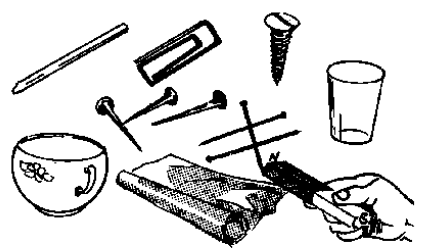
\includegraphics[width=0.4\textwidth]{./img/source/mag-non-mag.png}
\end{center}

\begin{description*}
%\item[Subtopic:]{}
\item[Materials:]{Magnets, various local objects e.g. nails, plastic, wood, cloth, copper, iron, aluminum, etc.}
%\item[Setup:]{}
\item[Procedure:]{Bring a magnet close to each of the materials listed above.}
%\item[Hazards:]{}
\item[Questions:]{What happens to each material?}
\item[Observations:]{Some materials such as nails and paper clips are attracted to the magnet, while others like toothpicks and plastic are not.}
\item[Theory:]{Materials that are attracted by magnets are called \emph{magnetic materials}, while those that are not attracted to magnets are called \emph{non-magnetic materials}.}
%\item[Applications:]{}
%\item[Notes:]{}
\end{description*}

%==================================================================================================%

\section*{Properties of Magnets}


\subsection{Interaction Between Magnets}

\begin{center}
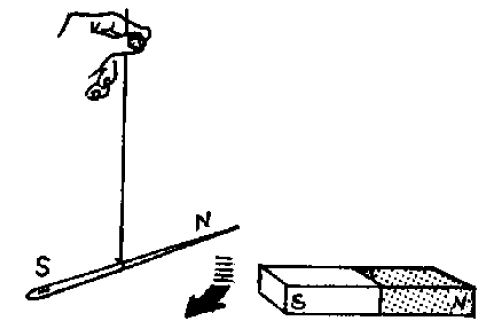
\includegraphics[width=0.4\textwidth]{./img/source/mag-interaction.png}
\end{center}

\begin{description*}
%\item[Subtopic:]{}
\item[Materials:]{2 magnets or magnetised needles}
%\item[Setup:]{}
\item[Procedure:]{Suspend one magnet or magnetised needle and bring the other close to it. First try N-pole to N-pole, then N-pole to S-pole, and so on.}
%\item[Hazards:]{}
%\item[Questions:]{}
\item[Observations:]{When two N-pols or two S-poles are placed near each other, the pin deflects away from the magnet, but when an N-pole and S-pole are near together, they attract.}
\item[Theory:]{Like poles repel, unlike poles attract.}
%\item[Applications:]{}
%\item[Notes:]{}
\end{description*}

%==================================================================================================%

\section*{Magnetisation}


\subsection{Stroking Method}

\begin{center}
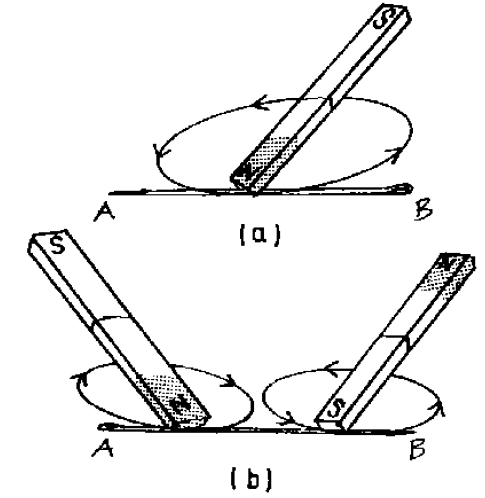
\includegraphics[width=0.35\textwidth]{./img/source/mag-stroke.png}
\end{center}

\begin{description*}
%\item[Subtopic:]{}
\item[Materials:]{Magnet, needle}
%\item[Setup:]{}
\item[Procedure:]{Move one pole of a bar magnet many times along the needle as shown in (a). Now take another needle and move the magnet as shown in (b), starting from the middle.}
%\item[Hazards:]{}
%\item[Questions:]{}
\item[Observations:]{The needle in (a) has a N-pole at A and S-pole at B, while the needle in (b) has a S-pole at A and a N-pole at B.}
\item[Theory:]{The first needle is magnetised by the single touch method, and the second is magnetised by the double touch method.}
%\item[Applications:]{}
%\item[Notes:]{}
\end{description*}

\subsection{Electromagnet}

\begin{center}
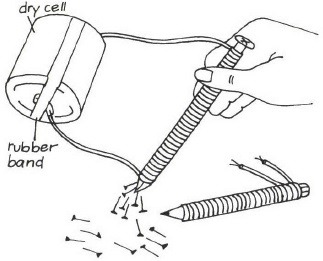
\includegraphics[width=0.35\textwidth]{./img/vso/electromagnet.jpg}
\end{center}

\begin{description*}
%\item[Subtopic:]{}
\item[Materials:]{Dry cell, nail, insulated copper wire, pins}
%\item[Setup:]{}
\item[Procedure:]{Make about 50 turns of wire around the nail. Connect the wire to the dry cell. Pick up the pins with the magnetised nail.}
%\item[Hazards:]{}
%\item[Questions:]{}
%\item[Observations:]{}
\item[Theory:]{The nail is magnetised by the electrical method. The moving electric charge in the wire solenoid creates a magnetic field in the nail. Strength of the magnet depends on the number of turns and current.}
%\item[Applications:]{}
%\item[Notes:]{}
\end{description*}

%==================================================================================================%

\section*{Demagnetisation}


\subsection{Demagnetisation of a Magnet}

\begin{center}
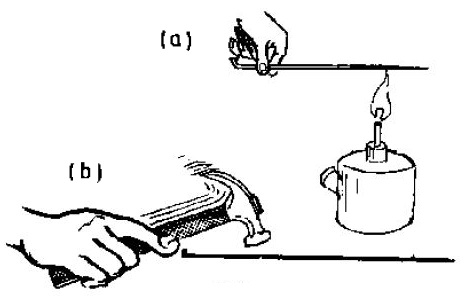
\includegraphics[width=0.45\textwidth]{./img/source/demagnetisation.jpg}
\end{center}

\begin{description*}
%\item[Subtopic:]{}
\item[Materials:]{Magnetised needles, paper clips, hammer, \nameref{sec:heatsources}}
%\item[Setup:]{}
\item[Procedure:]{Take two magnetised needles. Check to make sure they attract paper clips. Heat one needle in a flame (a) and hammer another several times (b). Check if the needles still retain their
magnetism.}
%\item[Hazards:]{}
%\item[Questions:]{}
\item[Observations:]{The magnetism of the needles is lost.}
\item[Theory:]{Magnets should not be kept in hot places or dropped or they may lose their
magnetism.}
%\item[Applications:]{}
%\item[Notes:]{}
\end{description*}

%==================================================================================================%

\section*{Magnetic Fields}


\subsection{Magnetic Filings} \index{Iron filings}

\begin{center}
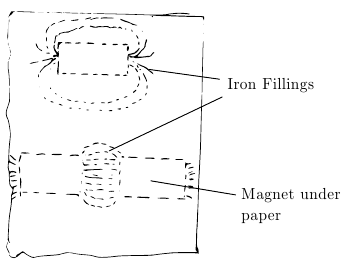
\includegraphics[width=0.45\textwidth]{./img/magnetic-fields.png}
\end{center}

\begin{description*}
%\item[Subtopic:]{}
\item[Materials:]{Bar magnets, paper, steel wool}
%\item[Setup:]{}
\item[Procedure:]{Place one or two bar magnets under a sheet of paper. Sprinkle iron filings over the top to reveal the lines of the magnetic field.}
%\item[Hazards:]{}
%\item[Questions:]{}
%\item[Observations:]{The iron filings reveal the magnetic lines of force.}
\item[Theory:]{Filings gather around the poles, where the magnetic force is strongest. Lines of repulsion are seen for like poles, and there is a \emph{neutral point} in the center through which no lines pass. Lines of attraction are shown for unlike poles.}
%\item[Applications:]{}
%\item[Notes:]{}
\end{description*}

\columnbreak

\subsection{Simple Compass} \index{Compass}

\begin{center}
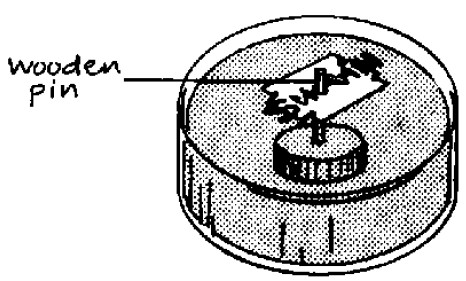
\includegraphics[width=0.35\textwidth]{./img/source/compass.png}
\end{center}

\begin{description*}
%\item[Subtopic:]{}
\item[Materials:]{Bowl filled with water, wooden pin, magnetised razor blade}
%\item[Setup:]{}
\item[Procedure:]{Fix a wooden pin vertically in a bowl of water. Slip a magnetised razor blade along the pin and carefully place it on the surface of the water so that it can rotate. Gently rotate the bowl and then the razor blade and observe what happens.}
%\item[Hazards:]{}
%\item[Questions:]{}
\item[Observations:]{When the bowl is rotated, the razor blade continues to lie in the N-S direction. When rotated itself, it returns to this orientation.}
\item[Theory:]{The magnetised razor blade aligns itself with earth's magnetic field in a N-S direction. As long as it remains magnetised, it will keep this orientation.}
%\item[Applications:]{}
%\item[Notes:]{}
\end{description*}

\subsection{Magnetic Dip Gauge}

\begin{center}
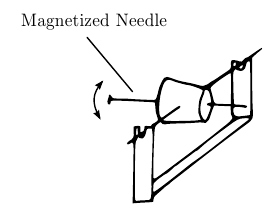
\includegraphics[width=0.35\textwidth]{./img/magnetic-dip-gauge.png}
\end{center}

\begin{description*}
%\item[Subtopic:]{}
\item[Materials:]{Magnet, needle, cork/foam, two pins, paper, pen, cardboard or metal strip}
\item[Setup:]{Push the two pins into the ends of the cork to create an axle. Push a needle through the cork perpendicular to the axle. Balance the pins on a U-shaped stand made of cardboard or metal strips.}
\item[Procedure:]{Set the gauge so that the needle is free to rotate vertically. Then magnetise the needle by stroking with a bar magnet.}
%\item[Hazards:]{}
%\item[Questions:]{}
\item[Observations:]{Before magnetising the needle, it balances horizontally in equilibrium. When magnetised however, it will dip down to show the direction of earth's magnetic field.}
\item[Theory:]{Like a compass, the needle naturally moves to show the direction of the earth's magnetic field. The gauge only works if facing N-S.}
%\item[Applications:]{}
%\item[Notes:]{}
\end{description*}

%==================================================================================================%




\end{multicols}

\pagebreak